\section{Applying Online-PCA}

\subsection{Novelty filter}

\mode<presentation>{
\begin{frame} 
    \begin{center} \huge
        \secname
    \end{center}
    Same as PCA
    Example Application: Novelty filter
\end{frame}
}

\begin{frame}

Applying online PCA for detecting outliers - identifying observations with unusual features. 

\begin{center}
	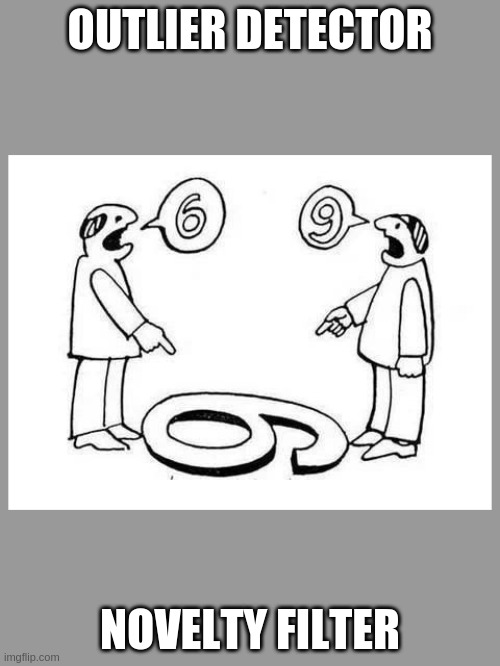
\includegraphics[width=0.3\textwidth]{img/meme_outlier_novelty}%
\end{center}

Can also be done using ``standard``/batch PCA

\end{frame}

\question{What are the PCs with smallest Eigenvalues useful for?}

\question{Can we modify online PCA by learning the PCs in reverse order (i.e. PCs with smallest eigenvalues first?}

\question{Is there an alternative way to learn a novelty filter? Under which assumptins does the alternative work?}

- (cf. slides 1.2 \#23-\#25.)

\section{PCA vs. online PCA}

\underline{Common properties:}

\begin{itemize}
\item assume the data is centered
\item sensitive to the scales of the individual variables
\item for stationary data, both converge to the same solution
\item limited to linear correlations between the variables (cf. Kernel PCA to account for non-linear correlations)
\end{itemize}

\question{PCA vs. online PCA. When do we use which?}

- staionarity of the data, can I fit all the data into memory?
